\problem{15}
The equilibrium condition for a system in contact with a reservoir,
and between coexisting phases (such as vapor and liquid),
requires that the temperature, pressure, and chemical potential are equal.
In this problem, we will examine how the nature of phase coexistence 
is affected by these conditions.

\smallskip \subp
The chemical potential of the liquid and vapor phases of a pure substance must be equal
($\mu_{\rm L} = \mu_{\rm V}$)
along its liquid-vapor coexistence curve in the $(p,T)$ plane. 
Using the Gibbs-Duhem relation, show that the following is true
for the saturation pressure and temperature:
\[ \frac{\dd p}{\dd T} = 
   \frac{\underline{S}_{\rm V} - \underline{S}_{\rm L}}
        {\underline{V}_{\rm V} - \underline{V}_{\rm L}} \]
$\underline{S}_{\rm V, L}$ and $\underline{V}_{\rm V, L}$ are the 
molar entropy and volume in the vapor and liquid phases, respectively.
\solution{\\
The Gibbs-Duhem relationship for a pure substance is 
$S \dd T - V \dd p + N \dd \mu = 0$. Rearrange:
\[ \dd \mu = -\frac{S}{N}\,\dd T + \frac{V}{N}\,\dd p 
           = -\underline{S}\,\dd T + \underline{V}\,\dd p \]
Along the coexistence curve, both $\mu_{\rm L} = \mu_{\rm V}$
{\bf and} $\dd \mu_{\rm L} = \dd \mu_{\rm V}$.
The second condition constrains our line in $(p,T)$ space to the coexistence curve.
Since $T$ and $p$ are equal for phases at equilibrium, 
$\dd \mu_{\rm L} = \dd \mu_{\rm V}$ can be rewritten:
\[  -\underline{S}_{\rm L}\,\dd T_{\rm sat} 
    +\underline{V}_{\rm L}\,\dd p_{\rm sat} 
  = -\underline{S}_{\rm V}\,\dd T_{\rm sat} 
    +\underline{V}_{\rm V}\,\dd p_{\rm sat} \]
With minor rearranging:
\[ -(\underline{V}_{\rm V} - \underline{V}_{\rm L})\,\dd p 
 = -(\underline{S}_{\rm V} - \underline{S}_{\rm L})\,\dd T \]
\[ \boxed{ \frac{\dd p_{\rm sat} }{\dd T_{\rm sat}} =
           \frac{\underline{S}_{\rm V}  
                -\underline{S}_{\rm L}}
                {\underline{V}_{\rm V} 
                -\underline{V}_{\rm L}} } \]
}



\smallskip \subp
Assume that along the coexistence curve, 
the latent heat of vaporization 
$L \equiv T(\underline{S}_{\rm V} - \underline{S}_{\rm L})$ 
is approximately constant.
In addition, assume that the molar volume of liquid 
is much smaller than vapor,
and that the vapor phase is well-described by the ideal gas law.
Show that, for any two points on the coexistence curve, the following is true:
\[ \ln(p_1/p_2) = \frac{L}{N_A k_{\rm B}} (1/T_2 - 1/T_1) \]
\solution{\\
Assuming that the vapor is ideal and 
$\underline{V}_{\rm V} \gg \underline{V}_{\rm L}$, 
$(\underline{V}_{\rm V} - \underline{V}_{\rm L}) \approx 
  \underline{V}_{\rm V} \approx \frac{\kT}{p}$. 
Substituting this in, along with the definition of the latent heat given
in the problem statement:
\[ \frac{T^2}{p} \frac{\dd p_{\rm sat} }{\dd T_{\rm sat}} 
 = -\frac{\dd \ln p}{\dd (1/T)} = \frac{L}{k_B} \]
This is the Clausius-Clapeyron equation, simplified for a low-pressure ideal gas.
Integrate:
\[ -\int_{p_1}^{p_2} \dd \ln p  
 = \frac{L}{k_B} \int_{T_1}^{T_2} \dd \left( \frac{1}{T} \right) \]
\[ \boxed{ \ln (p_1/p_2) = \frac{L}{k_B} \left( \frac{1}{T_2} - \frac{1}{T_1} \right) } \]
}
\smallskip \subp
Look up a few ($\sim5$) data points, $(T_\text{sat}, p_\text{sat})$, 
for the saturation temperature and pressure of water.
Using part (b), estimate the latent heat of
vaporization for water using your data.
\solution{ \\
The best way to do this is to use:
\[ \frac{\dd \ln p_{\rm sat}}{\dd (1/T_{\rm sat})} = - \frac{L}{k_{\rm B}} \]
Simply plot $\ln p_{\rm sat}$ against $T_{\rm sat}^{-1}$.
The latent heat can be estimated directly from the slope.
We did not check your values unless something seemed exceedingly wrong.
}

\smallskip \subp
Vapor pressure near a liquid droplet is larger than
it would be near a bulk liquid  due to surface tension effects. 
Using a chemical potential balance, show that near a spherical droplet:
\[\underline{V}_{\rm L} 
  \left(P^{\rm (sat)}_{\rm droplet} - P^{\rm (sat)} + \frac{2\gamma}{r} \right)
 = R T \ln\left( \frac{P^{\rm (sat)}_{\rm droplet}}{P^{\rm (sat)}} \right) \]
Here $\underline{V}_{\rm L}$ is the molar volume of liquid,
$\gamma$ is the interfacial tension,
and $r$ is the droplet radius.
You may assume $\underline{V}_{\rm L}$ is constant
at the pressures used in this problem.
{\bf State clearly any assumptions made in your derivation}.
\solution{\\
The most straightforward way to do this is to apply
the Gibbs-Duhem relationship.
\[ \dd \mu = -\frac{S}{N}\,\dd T + \frac{V}{N}\,\dd p 
           = -\underline{S} \dd T + \underline{V} \dd p \]
We would like to use bulk liquid as a reference state.
Assume that there is no pressure drop across the interface
in a bulk liquid, i.e.
$p^{\rm (sat)}_{\rm V, bulk} = p^{\rm (sat)}_{\rm L, bulk} 
                             = p^{\rm (sat)}$.
From this point on, we use $p^{\rm (sat)}$ to refer
to the bulk saturation pressure, and $p_{\rm L}$ and $p_{\rm V}$
to refer to the droplet saturation pressure
in the liquid and vapor phases, respectively.
Using Gibbs-Duhem, we can write:
\[ \mu_{\rm L} (p_{\rm L},T) - \mu_{\rm L} (p^{\rm (sat)},T) 
 = \int_{p^{\rm (sat)}}^{p_{\rm L}} \underline{V}_{\rm L}\,\dd p \]
\[ \mu_{\rm V} (p_{\rm V},T) - \mu_{\rm V} (p^{\rm (sat)},T) 
 = \int_{p^{\rm (sat)}}^{p_{\rm V}} \underline{V}_{\rm V}\,\dd p \]
Now, assume that the vapor phase behaves as an ideal gas, and that
the liquid is incompressible:
\[ \mu_{\rm L} (p_{\rm L},T) - \mu_{\rm L} (p^{\rm (sat)},T) 
 = \underline{V}_{\rm L} \int_{p^{\rm (sat)}}^{p_{\rm L}} \dd p 
 = \underline{V}_{\rm L} \left( p_{\rm L} - p^{\rm (sat)}\right) \]
\[ \mu_{\rm V} (p_{\rm V},T) - \mu_{\rm V} (p^{\rm (sat)},T) 
 = \int_{p^{\rm (sat)}}^{p_{\rm V}} \frac{RT}{p}\,\dd p 
 = RT \ln \left( \frac{p_{\rm V}}{p^{\rm (sat)}} \right) \]
The chemical potentials of the liquid and vapor phases
must be equal at equilibrium. 
Both of our reference chemical potentials must be identical, 
so setting $\mu_{\rm L} (p_{\rm L},T) = \mu_{\rm V} (p_{\rm V},T)$:
\[ \underline{V}_{\rm L} \left( p_{\rm L} - p^{\rm (sat)}\right) 
 = RT \ln \left( \frac{p_{\rm V}}{p^{\rm (sat)}} \right) \]
In HW2, we showed that the pressure drop across a spherical droplet
was given by $p = 2 \gamma/r$, 
where $p$ was the pressure inside minus the pressure outside. Thus:
\[ p_{\rm L} = p_{\rm V} + \frac{2 \gamma}{r} \]
If we rewrite $p_{\rm V} = p^{\rm (sat)}_{\rm droplet}$, we recover:
\[ \boxed{ \underline{V}_{\rm L} \left( p^{\rm (sat)}_{\rm droplet}
         - p^{\rm (sat)} + \frac{2 \gamma}{r} \right) 
         = RT \ln \left( \frac{p^{\rm (sat)}_{\rm droplet}}
                              {p^{\rm (sat)}} \right) } \]
}
\smallskip \subp
If we assume $P^{\rm (sat)}_{\rm droplet} - P^{\rm (sat)} \approx 0$,
then the expression in part (d) simplifies to:
\[ P^{\rm (sat)}_{\rm droplet} = P^{\rm (sat)} 
  \exp\left( \frac{2\gamma \underline{V}_{\rm L}}{r RT} \right) \]
Under what conditions is this assumption valid?
Calculate the deviation in vapor pressure (relative to bulk liquid)
near a water droplet with radius {\rm 5\,mm} at room temperature.
%The opposite effect is expected in porous materials)
\solution{\\
The assumption is valid when:
 \[ p^{\rm (sat)}_{\rm droplet} - p^{\rm (sat)} \ll \frac{2 \gamma}{r} \]
It is more informative to self-consistently verify the simplified form.
Our condition is valid when the exponential is near one -- 
that is, when the argument to the exponential is very small.
Define $p_\gamma = 2\gamma/r$ as the pressure drop due to surface tension.
Since we have assumed the vapor is ideal, 
$p^{\rm (sat)}_{\rm droplet} = RT/\underline{V}_{\rm V}$.
The condition becomes:
\[ \frac{2 \gamma \underline{V}_{\rm L}}{r RT}
 = \left( \frac{\underline{V}_{\rm L}}{\underline{V}_{\rm V}} \right)  
   \left( \frac{p_\gamma}{p^{\rm (sat)}_{\rm droplet}} \right) \ll 1\]
It is difficult to estimate the second ratio;
however, the first ratio indicates assumption is valid
when $\underline{V}_{\rm V} \gg \underline{V}_{\rm L}$, 
which is typically true.
\[ \boxed{\text{Assumption is valid when } 
          \underline{V}_{\rm V} \gg \underline{V}_{\rm L} } \]
Let us calculate the deviation in vapor pressure for a physical system.
Using $\gamma = 72\,{\rm mN}/{\rm m}$:
\[ \frac{P^{\rm (sat)}_{\rm droplet}}{P^{\rm (sat)}} 
 = \exp \left( 
        \frac{2 * 0.072 * 1.8*10^{-5} \,\text{N}\text{ m}^2\text{ mol}^{-1}}
             {0.005*8.31*300\,\text{N}\text{ m}^2\text{ mol}^{-1}} \right)
 = \exp \left( 2*10^{-7} \right) \approx 1 \]
Therefore, for a $5\,{\rm mm}$ water droplet at the given conditions:
\[ \boxed{ p^{\rm (sat)}_{\rm droplet} \approx p^{\rm (sat)} } \]
\newpage
}

\bigskip
\problem{15}
Equations of state for non-ideal fluids may be analyzed by studying
the compressibility factor $Z\equiv pv/(RT)$,
where $v$ is the molecular molar volume $V/N$.
The virial expansion for $Z$ is defined as
$$Z = 1 + \frac{B_2}{v} + \frac{B_3}{v^2} + \cdots$$
where $B_2$, $B_3$, $\ldots$ are called the second, the third, 
$\ldots$ virial coefficients, respectively.
These coefficients can be related to intermolecular interactions.

\smallskip
\subp
Find the second and the third virial coefficents for a Van der Waals fluid with an equation of state 
$p = RT/(v - b) - a / v^2$.
\solution{
\begin{align*}
  Z &\equiv \frac{pv}{RT} = p \left( \frac{v}{RT} \right) 
          = \left( \frac{RT}{v-b} - \frac{a}{v^2} \right) \left( \frac{v}{RT} \right) \\
         &= \frac{v}{v-b} - \frac{a}{RTv} 
          = \frac{1}{1-b/v} - \left( \frac{a}{RT} \right) \frac{1}{v}
\end{align*}
The ratio $b/v$ is the excluded volume (hard-sphere volume) of a gas molecule 
divided by the molecular molar volume $v \equiv V/N$. 
In a gas, it's safe to assume this quantity is very small. 
Therefore, we use a Taylor expansion to approximate this term:
\[ \frac{1}{1-b/v} \approx 1 + \frac{b}{v} + \frac{b^2}{v^2} \cdots \]
Plugging this into the expression for $Z$ yields:
\[ Z = 1 + \left( b - \frac{a}{RT} \right) \frac{1}{v} + b^2 \frac{1}{v^2} + \cdots \]
Thus, using the approximation $b \ll v$, the second and third virial coefficients are:
\[ \boxed{ B_2 = b - \frac{a}{RT} } \]
\[ \boxed{ B_3 = b^2 } \]
}

\smallskip
\subp
 The second virial coefficient is related to the pairwise inter-molecular potential $u(r)$ via
\[ B_2 = 2\pi \NA \int_0^\infty\left[1 - \exp\left(-\frac{u(r)}{\kT}\right)\right] r^2 \dd r. \]
%In the ``hard-sphere'' model, the interaction potential between two molecules is given by
%\begin{equation*}
%\Gamma(r) = \left\{\begin{aligned}
%     0,\quad& r\ge d, \\
%\infty,\quad& 0 < r < d.
%\end{aligned}\right.
%\end{equation*}
At short distances, the intermolecular potential is dominated by repulsion.
Assume $u(r)$ is given by $u(r) = c\, r^{-n} \, (n>3)$, where $c$ is a positive constant.
Show that $B_2$ will have the form:
\begin{equation*}
B_2 = \frac{2\pi \NA}{3} \left(\frac{c}{\kT}\right)^{3/n} \Gamma(1-3/n)
\end{equation*}
The gamma function is defined as
$\Gamma(z) \equiv \int_{0}^\infty\!\dd x\, e^{-x} x^{z-1} $. 
\smallskip {\bf Hint}: {\sl Try integrating by parts}.
\solution{\\
Integrate by parts ($\int u \dd v = uv - \int v \dd u$)
with $u = 1 - \exp \left( \frac{-cr^{-n}}{\kT} \right)$ 
and $dv = r^2 \dd r$:
\begin{align*}   
   \frac{B_2}{2\pi N_A} &= \left[ \frac{r^3}{3} - \frac{r^3}{3} \exp 
      \left( - \frac{cr^{-n}}{k_B T} \right) \right]^{\infty}_0
    - \int_0^\infty \frac{r^3}{3} \left[ \frac{n c}{k_B T} r^{-n-1} 
      \exp \left( - \frac{cr^{-n}}{k_B T} \right) \right] \dd r \\
    &=  \left( 0 - 0 \right) - \frac{1}{3} \int_0^\infty r^3 
        \exp \left( - \frac{cr^{-n}}{k_B T} \right) 
             \left( \frac{cnr^{-n-1}}{k_B T}\,\dd r \right) \\
    &= \frac{1}{3} \int_0^\infty r^3 \exp \left( - \frac{cr^{-n}}{k_B T} \right) 
        \dd \left( \frac{cr^{-n}}{k_B T} \right) \\ 
\end{align*}
This suggests the need for the following substitution:
\[ x = \frac{cr^{-n}}{k_B T} \qquad \qquad
   r = \left( \frac{k_B T x}{c} \right)^{-1/n} \]
Based on this definition, $r^{-n} = \kT x / c$:
\begin{align*}
   B_2 &= \frac{2 \pi N_A}{3} \int_0^\infty 
          \left( \frac{k_B T x}{c} \right)^{-3/n} e^{-x} dx \\
       &= \frac{2 \pi N_A}{3} \left( \frac{c}{k_B T} \right)^{3/n} 
          \int_0^\infty - x^{3/n} e^{-x} dx \\
\end{align*}
Let $z \equiv 1 - 3/n$. We can write $x^{3/n} = x^{z - 1}$ and apply the
gamma function definition:
\[ \boxed{ B_2 = \frac{2\pi N_A}{3} \left( \frac{c}{\kT} \right)^{3/n} \Gamma (1 - 3/n) } \]
}


\smallskip \subp
The pairwise Lennard-Jones potential
leads to the Van der Waals equation of state.
It has the form $u(r) = \epsilon \left[ (\sigma/r)^{12} -  (\sigma/r)^6 \right]$,
where $\epsilon$ and $\sigma$ are parameters denoting the 
strength and range of the interaction.
Show that (i), the second virial coefficient can be approximated by
\[ B_2 \simeq \frac{2\pi \NA \sigma^3}{3} \left(1 - \frac{\epsilon}{\kB T} \right)\,,\]
and (ii) determine the values of $a$ and $b$ in the Van der Waals equation of state. 
\smallskip {\bf Hint}: {\sl Consider the $r < \sigma$ and $r > \sigma$ regimes separately}.
\solution{\\
\[ \frac{B_2}{2\pi N_A} = 
   \int_0^\infty \left[ 1 - \exp \left( \frac{-\epsilon}{\kT} 
   \left[ (\sigma/r)^{12} - (\sigma/r)^{6} \right] \right) \right] r^2 \dd r \]
Let us define $x \equiv (\sigma/r)^6$. 
We can approximate the integral by splitting it up into two regimes.
\[ \frac{B_2}{2\pi N_A} = 
   \int_0^\sigma \left[ 1 - \exp \left( 
   \frac{-\epsilon x (x-1)}{\kT} \right) \right] r^2 \dd r 
 + \int_\sigma^\infty \left[ 1 - \exp \left( 
   \frac{-\epsilon x (x-1)}{\kT} \right) \right] r^2 \dd r\]
In this first integral, $r < \sigma$ so we expect $x \gg 1$.
The argument to the exponential is thus a very large negative number,
and so the exponential is approximately zero in this regime.
In the second integral, $r > \sigma$ and $x \ll 1$. 
Thus, $\exp \left( \frac{-\epsilon x(x-1)}{\kT} \right) \approx
       \exp \left( \frac{\epsilon x}{\kT} \right)$.
We Taylor expand under the assumption that $x$ is very small:
\[(x \ll 1) \quad : \quad \exp \left( \frac{\epsilon x}{\kT} \right)
  \approx 1 + \frac{\epsilon x}{\kT} \]
These approximations break down near $r \approx \sigma$, 
but that is why our $B_2$ will be approximate.
\begin{align*}
\frac{B_2}{2\pi N_A} &\approx \int_0^\sigma \left[ 1 - 0 \right] r^2 \dd r
   + \int_\sigma^\infty \left[ 1 - 1 - \frac{\epsilon x}{\kT} \right] r^2 \dd r \\
  &= \left[ \frac{\sigma^3}{3} - 0 \right] 
   - \int_\sigma^\infty \left[ \frac{\epsilon \sigma^6}{\kT r^4} \right] \dd r \\
  &= \frac{\sigma^3}{3} + \left[ \frac{\epsilon \sigma^6}{3 \kT r^3} \right]_\sigma^\infty 
   = \frac{\sigma^3}{3} + \left[ 0 - \frac{\epsilon \sigma^3}{3 \kT} \right]
\end{align*}
Factoring out $\sigma^3/3$, we arrive at:
\[ \boxed{ B_2 \simeq \frac{2\pi N_a \sigma^3}{3} 
           \left( 1 - \frac{\epsilon}{\kT} \right) }\]
From part (a), we know that $B_2 = b - \frac{a}{RT} = b - \frac{a N_A}{\kT}$. 
Matching terms, it is clear that:
\[ \boxed{ a = \frac{2 \pi \sigma^3 \epsilon}{3} } \]
\[ \boxed{ b = \frac{2 \pi N_A \sigma^3}{3} } \]
\newpage
}

\bigskip
\problem{12}
A drop of ink spreading in solution can be modeled using the diffusion equation.
The Dirac delta function is often used as an initial condition --
this represents the highly concentrated ink drop at $t = 0$. 
\begin{align*}
\text{(1D diffusion):} \quad \frac{\partial c(x,t)}{\partial t}
   = D \frac{\partial^2 c(x,t)}{\partial x^2}
     \qquad &, \qquad c(x,t=0) = \delta(x) \\
\text{(3D diffusion):} \quad \frac{\partial c({\bf r},t)}{\partial t} 
   = D \nabla^2 c({\bf r}, t)
     \qquad &, \qquad c({\bf r},t=0) = \delta^3({\bf r}) 
\end{align*}
${\bf r} \equiv \{x,y,z\}$ and $\delta^3({\bf r}) \equiv \delta(x) \delta(y) \delta(z)$.
You may find the following Gaussian integral identities helpful:
\[ \int_{-\infty}^\infty e^{-ax^2 + bx}\,\dd x = 
   \sqrt{\frac{\pi}{a}}\,e^\frac{b^2}{4a} \]
\[ \int_{-\infty}^\infty x^2 e^{\frac{-x^2}{a}}\,\dd x =
   \frac{\sqrt{\pi a^3}}{2} \] 
   
\smallskip \subp
Solve (i) the 1D diffusion equation and (ii) the 3D diffusion equation
for the concentration $c$. 
\solution{\\
Solving the PDE with a Fourier transform is a good idea. 
We prefer the following convention:
\[ \hat{f}(k) = \int_{-\infty}^{\infty} \dd x\, f(x) e^{-\img kx} \]
\[ f(k) = \frac{1}{2\pi} \int_{-\infty}^{\infty} \dd k\, \hat{f}(k) e^{\img kx} \]
Taking the Fourier transform of the PDE converts it to a 1$^\text{st}$ order ODE:
\[ \frac{\partial \hat{c}(k,t)}{\partial t} = -D k^2 \hat{c}(k,t) 
   \qquad , \qquad \hat{c}(k,t=0) = 1 \]
\[ \hat{c}(k,t) = e^{-Dk^2t} \]
Transform back to real space by applying Gaussian integral identities:
\[ c(x,t) = \frac{1}{2\pi} \int_{-\infty}^{\infty} \dd k\,e^{-Dk^2t + \img k x} 
          = \frac{1}{2\pi} \sqrt{\frac{\pi}{Dt}}\,e^\frac{(\img x)^2}{4 Dt} 
          = \frac{e^\frac{-x^2}{4Dt}}{2 \sqrt{\pi D t}} \]
For the 3D case, the procedure is nearly identical.
Adopting the standard vector notation 
${\bf r} = \{x,y,z\}$ and ${\bf k} = \{k_x,k_y,k_z\}$,
the Fourier-space solution is the same:
\[ \hat{c}({\bf k},t) = e^{-D|{\bf k}|^2t} = e^{-D k_x^2 t - D k_y^2 t - D k_z^2 t} \]
The real-space solution in 3D is just the product of three 1D solutions:
\[ \hat{c}({\bf r},t) = c(x,t) c(y,t) c(z,t) 
                      = \left( \frac{1}{2 \sqrt{\pi D t}} \right)^3
                        e^\frac{-x^2-y^2-z^2}{4Dt} \]
\[ \boxed{c(x,t) = \frac{1}{2 \sqrt{\pi D t}}\,e^\frac{-x^2}{4Dt} } \]
\[ \boxed{c({\bf r},t) = \left( \frac{1}{2 \sqrt{\pi D t}} \right)^3\,
                         e^\frac{-|{\bf r}|^2}{4Dt} } \]
}

\smallskip \subp
The concentration $c(x,t)$ can be interpreted as the probability of
observing an ink molecule at position $x$ and time $t$.
Using this probability distribution, compute the 
rate of change in entropy $\dot S(t) = \frac{\dd S(t)}{\dd t}$
for (i) 1D diffusion and (ii) 3D diffusion.
\solution{\\
The concentration is already normalized by the initial condition; 
that is, $\int_{-\infty}^\infty \dd x\,c(x,t) = 1$ 
(evaluate the integral if you're not convinced).
Thus, we can substitute it in directly for the probability.
Using the Gibbs' definition of entropy (1D case): 
\[ S(t) = -k_B \sum_j p_j \ln p_j = -k_B \int_{-\infty}^\infty\dd x\,c(x,t) \ln c(x,t) \]
For convenience, let $A \equiv \left( \sqrt{4 \pi Dt} \right)^{-1}$.
\begin{align*}
  S(t) &= -k_B \int_{-\infty}^\infty\dd x\, A e^\frac{-x^2}{4Dt} 
          \left(\ln A - \frac{x^2}{4Dt} \right)
        = -k_B A \ln A \int_{-\infty}^\infty\dd x\,e^\frac{-x^2}{4Dt} 
          +k_B \frac{A}{4Dt} \int_{-\infty}^\infty \dd x\,x^2\,e^\frac{-x^2}{4Dt} \\
       &= -k_B A \ln A \left( \sqrt{4 \pi D t} \right) 
          +k_B \frac{A}{4Dt} \left( \frac{\sqrt{\pi (4Dt)^3}}{2} \right)
        = -k_B A (\sqrt{4 \pi D t}) \left[ \ln A - \frac{1}{2} \right] \\
       &= -k_B \left[ \ln A - \frac{1}{2} \right]
        = k_B \left[ \ln(\sqrt{4 \pi D t}) + \frac{1}{2} \right] 
        = k_B \left[ \frac{1}{2} \ln (4 \pi D t) + \frac{1}{2} \right]
\end{align*}
The time derivative is straightforward.
The rate of entropy change for the 1D case is given by:
\[ \boxed{\text{1D case : } \dot{S}(t) = \frac{k_B}{2t} } \]
The 3D solution is the product of three independent 1D solutions.
\begin{align*}
  S(t) &= -k_B A^3 \iiint_V \dd x\,\dd y\,\dd z\,e^\frac{-x^2-y^2-z^2}{4Dt}
          \left(3 \ln A - \frac{x^2 + y^2 + z^2}{4Dt} \right) \\ 
       &= -3 k_B A^3 \ln A \left( 4\pi D t \right)^{3/2}
        + \frac{k_B A^3}{4 D t} \left(3 \frac{\sqrt{\pi (4Dt)^3}}{2} \right) \\
       &= -k_B A^3 (4\pi D t)^{3/2} \left[ 3 \ln A - \frac{3}{2} \right] \\
       &= 3 k_B \left[ \ln \left( \sqrt{4 \pi D t} \right) + \frac{1}{2} \right]
        = k_B \left[ \frac{3}{2} \ln (4 \pi D t) + \frac{3}{2} \right]
\end{align*}
As expected, this is just three times the entropy of the 1D case.
Therefore:
\[ \boxed{\text{3D case : } \dot{S}(t) = \frac{3 k_B}{2t} } \]
}

\smallskip \subp
What happens to $\dot S(t)$ as $t \to \infty$?
How does $\dot S(t)$ differ between 1D and 3D diffusion?
\solution{ \\
The rate of entropy generation approaches zero asymptotically as $t \to \infty$. 
Entropy is generated three times faster in the 3D case than the 1D case,
commensurate with the number of dimensions available for the random walk.
\newpage
}

\bigskip
\problem{3}
C.E. Shannon (1948) perceived that entropy quantifies
the uncertainty in possible observations of a system,
and showed that Gibbs' entropy expression can be used to
calculate this ``uncertainty'':
\[ I = - \sum_n p_n \log_2\, p_n \]
Here $n$ denotes one of the possible outcomes of a single measurement,
and $p_n$ is its corresponding probability.
$I$ is the average information, in units of {\bf bits},
obtained from a single observation/measurement. 
(Shannon used the base-2 log for information, whereas entropy uses base-$e$).
\iffalse
For the two-state model we studied in class,
using the above notation, we may say that at $T = +\infty$,
the information collected after measuring the energetic state of a single particle is
$$I(\text{two state}; T=+\infty) = -\frac{1}{2}\log_2\left(\frac{1}{2}\right)
- \frac{1}{2}\log_2\left(\frac{1}{2}\right) = 1 \,\text{bit},$$
as the particle sits in any of the two states with probability $1/2$.
At zero temperature ($T=+0$), measuring the state of particles provides 0\,bit of information,
since we know with certainty before any measurement that the
particles are all seated in the low-energy state (the third law). \\
\fi
Shannon applied this analysis to the English language -- 
he noticed that the frequency of English words closely follows Zipf's law
(see Fig.~\ref{fig:zipf}):
$$ p_n = \frac{0.1}{n} .$$
Then he assumed that English language only has $n_\text{max} = 12367$ words.
This is obviously an irritating assumption, but it is required to ensure
$\sum_{n=1}^{n_\text{max}} \frac{0.1}{n} = 1.000$.
This assumption essentially neglects the entropy from rarely used words.
Based on this assumption, compute the average number of 
information bits $I$ per English word
(On average, there are $5.1$ letters per word in modern English).
For the average word, how many information bits $I$ are there per letter? 
As a reference, computers use 8 bits to store a single letter.

\begin{figure}[h]\centering
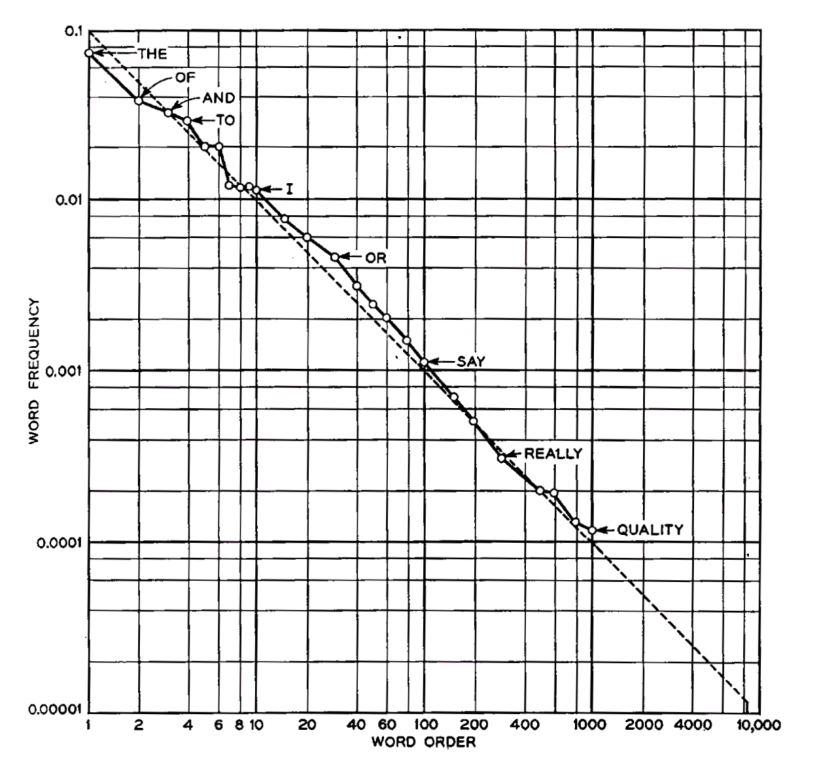
\includegraphics[width=0.45\textwidth,height=!]{zipf}
\caption{\label{fig:zipf}
Probability against frequency rank for English words.
The dashed line is the prediction of Zipf's law.
The most frequently used word is {\sl the};
the following ones are {\sl of}, {\sl and}, {\sl to}, etc.
}
\end{figure}

\solution{
This one is pretty straightforward. Given that $p_n = \frac{0.1}{n}$, and that $n = 1,2,\cdots,12367$:
\[ I = -\sum_{n=1}^{12367} \frac{0.1}{n} \log_2 \frac{0.1}{n} = 9.7 \text{ (using MATLAB)} \]
Note you could also approximate this with an integral.
It's not a great approximation, but it's close enough:
\[ I \approx \int_1^{12367} \frac{0.1}{n} \log_2 \frac{0.1}{n}\,\dd n = 9.5 \]
Either way, you can just divide $I$ by the average number of letters per word, $5.1$,
to approximate the number of bits per English word.
\[ \boxed{ \frac{I}{\text{word}} = 9.7\,\text{bits} \qquad , \qquad 
           \frac{I}{\text{letter}} = 1.9\,\text{bits} } \]
\newpage
}

\bigskip
\problem{6}
Suppose we have an ensemble of $m$ identical subsystems.
As an example, the diagram below illustrates the case of $m=8$ subsystems. 
In this problem, we are interested in the behavior of the ensemble
as $m \rightarrow \infty$. \\ \par
\centerline{\includegraphics[width=0.4\textwidth,height=!]{subsystem}}\smallskip
\noindent Each subsystem $i$ has an internal energy $E_i$ that fluctuates over time.
The statistical average and variance of subsystem energy, 
$\ave{E_i} \equiv \epsilon_i = \epsilon$ and
$\ave{(E_i - \ave{E_i})^2} \equiv \sigma^2_i = \sigma^2 $,
are the same for each subsystem.
Assume the subsystems are large enough such that boundary effects can be neglected.
Define the ensemble energy:
\[ E = \sum_{i=1}^m E_i \] 
Assuming energy fluctuations in different subsystems are uncorrelated,
show that the noise-to-signal ratio for $E$,
the total energy in the ensemble, scales with $1/\sqrt{m}$.
Specifically, we would like you to show that:
\[ \frac{\ave{(E - \ave{E})^2}^{1/2}}{\ave{E}} \propto \frac{1}{\sqrt{m}}\, \]
This ratio vanishes in the thermodynamic limit, $m\to\infty$.
This can be proven for all extensive quantities. 

\solution{ \\
For notational simplicity, let us define $\delta E \equiv E - \ave{E}$,
the deviation (from the mean) in ensemble energy, $E$.
\[ \ave{ \left( E - \ave{E} \right)^2 } = \ave{ \delta E^2 } 
 = \ave{ \left( \sum_i^m \delta E_i \right)^2 } 
 = \ave{ \sum_i^m \delta E_i \sum_j^m \delta E_j } \]
We need a different index for each summation here because
multiplication is distributive over sums.
Split the summation into `like'-terms and `unlike'-terms:
\[ \ave{ \sum_i^m \delta E_i \sum_j^m \delta E_j } 
 = \ave{ \sum_{i,j}^{m^2} \delta E_i \delta E_j } 
 = \ave{ \sum_i^m (\delta E_i)^2 } + \ave{ \sum_{i \neq j}^{m(m-1)} \delta E_i \delta E_j } \]
Try writing out the entire product of summations for $i,j = 3$ 
if you cannot make sense of the notation.
The summation over $i \neq j$ is the cross-correlation
in energy fluctuations between {\bf different} subsystems.
Assume this term is zero.
\[ \ave{ \sum_i (\delta E_i)^2 } + \ave{ \sum_{i \neq j}^{m(m-1)} 
   \delta E_i \delta E_j } 
  = m \ave{(\delta E_i)^2} = m \ave{ (E_i - \epsilon)^2 } = m \sigma^2 \]
We have taken advantage of the fact that the variance in subsystem energy 
$E_i$ is the same for each subsystem 
(this lets us factor out the $m$, 
since all the summation terms are the same). 
Now, we just need $\ave{E}$:
\[ \ave{E} = \ave{\sum_{i=1}^m E_i } = \sum_{i=1}^m \ave{E_i} = m \epsilon \]
Again, we were given the average energy of each subsystem is the same.
The signal to noise ratio is then:
\[ \boxed{ \frac{\ave{(E - \ave{E})^2}^{1/2}}{\ave{E}} 
         = \frac{\sqrt{m \sigma^2}}{m \epsilon} 
         = \frac{\sigma}{\sqrt{m} \epsilon } \propto \frac{1}{\sqrt{m}} } \]
}